\documentclass{beamer}
\usepackage{ctex}
\usepackage[export]{adjustbox}
\usepackage{listings}
\usepackage{xcolor}

\usetheme{focus}

\definecolor{codegreen}{RGB}{50 200 50}
\definecolor{codeblue}{RGB}{50 50 200}
\definecolor{codered}{RGB}{200 50 50}
\tikzset{
    global scale/.style={scale=#1,every node/.append style={scale=#1}},
    CC1/.style ={circle,minimum width = 30pt, minimum height =30pt, draw=black},
    CC2/.style ={circle,minimum width = 30pt, minimum height =30pt, draw=black, fill=blue!20},
    RA1/.style ={rectangle,minimum width = 30pt, minimum height =20pt, draw=black},
    RA2/.style ={rectangle,minimum width = 1cm, minimum height = 1cm, draw=black}
}

\title{算法分析与设计II}
\subtitle{2022-2023-2}
\date{Last Modified: 2023.1.16}
\institute{\vspace{2em} 数学与计算机学院 \\ 数据科学与大数据技术}
\titlegraphic{\vspace{5em} 
\includegraphics[scale=0.3]{fig/jlnu.pdf}}

\lstset{
    columns=flexible,       
    numbers=left,  
    numberstyle=\footnotesize\color{darkgray},  
    frame=shadowbox, 
    rulesepcolor= \color{gray}, 
    keywordstyle=\color{codeblue},         
    commentstyle=\color{codegreen},  
    stringstyle=\color{codered}, 
    showstringspaces=false,  
    xleftmargin=3em,
    xrightmargin=1em,              
    language=c++                           
}

\tikzset{
    CC1/.style ={
    circle,
    minimum width = 30pt, 
    minimum height =30pt, 
    draw=black
    }
}

\begin{document}
\frame{\titlepage}
\section{5. 贪心算法}
\begin{frame}{5.1 基础贪心算法问题}
    \begin{itemize}
        \item \textcolor{blue}{贪心算法}(greedy algorithm)的基本思路:在一个决策序列中,每一步单独的决策其优劣有一个度量标准来衡量;每一步决策总是选择在度量标准下最优的那个分支(决定);每一步决策一旦决定便不再更改(不同于回溯算法)
        \item \textcolor{blue}{排序}是贪心算法的基本操作,掌握系统的排序函数是必要条件
        \item 因为贪心算法并没有枚举所有情况,所以效率比较高,但是必须保证算法的正确性
        \item 背包问题也可以使用贪心算法来解,但是通常使用动态规划的方法
        \item 字符串中的\textcolor{blue}{哈夫曼编码},图算法中的\textcolor{blue}{最小生成树}采用的都是贪心算法的思想
    \end{itemize}
\end{frame}
\begin{frame}{2069 -- Super Star (poj.org)}
    \begin{itemize}
        \item \textcolor{blue}{最小包围球}(Smallest bounding sphere):将星星看作空间中的点,求包含所有给定星星的最小球体
        \vfill
        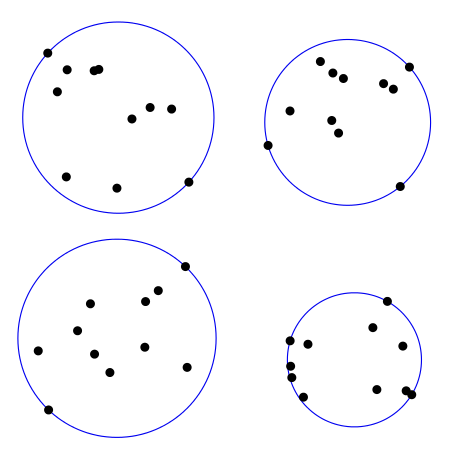
\includegraphics[width=0.2\textwidth,right]{fig/5-1.png}
    \end{itemize}
    \begin{block}{模拟退火法(SA,Simulated annealing)}
        \quad 一种通用概率算法,通过模拟金属退火的过程,在一定时间内寻找在一个很大搜寻空间中的近似最优解
    \end{block}
    \begin{itemize}
        \item 选取开始点,进行多轮迭代,每次在当前状态附近随机生成解空间,在解空间中选择最优的进行下一轮迭代,最终使得结果收敛到最优解附近结束
    \end{itemize}
\end{frame}
\begin{frame}{5.2 区间覆盖问题}
    \begin{itemize}
        \item 贪心算法的一类应用就是\textcolor{blue}{区间覆盖问题},这些问题共有的特征是给出一些具有左右端点的线段(\textcolor{blue}{区间}),这些线段存在于一个给定的区间内,在这个区间内求不同的覆盖问题
        \begin{enumerate}[(1)]
            \item 最大不相交线段数:在区间内找到尽可能多的线段,线段彼此之间不重叠
            \item 区间完全覆盖:找到最少的线段,完全覆盖给定的区间
            \item 区间选点问题:找到最少的点,使得每个线段中至少包含一个点
            \item 线段覆盖问题:找到最少的线段,覆盖所有的线段
            \item 线段重叠问题:将重叠的线段连接到一起,计算合并后线段的数量
        \end{enumerate}
    \end{itemize}
\end{frame}
\begin{frame}{1089 -- Intervals (poj.org)}
    \begin{itemize}
        \item There is given the series of $n$ closed intervals $[a_i; b_i]$, where $i=1,2,...,n$. The sum of those intervals may be represented as a sum of closed pairwise non-intersecting intervals.
        \item The task is to find such representation with the minimal number of intervals. 
        \item The intervals of this representation should be written in the output file in acceding order. We say that the intervals $[a; b]$ and $[c; d]$ are in ascending order if, and only if $a \leq b < c \leq d$.
    \end{itemize}
\end{frame}    
\begin{frame}{分析}
    \begin{columns}
        \column{0.3\textwidth}
            \begin{table}
                \begin{tabular}{cc}
                Input \\\hline
                5  & 6 \\\hline
				1  & 4  \\\hline
				10 & 10 \\\hline
				6  & 9  \\\hline
				8  & 10  \\\hline
                \end{tabular}
            \end{table}
            \begin{table}
                \begin{tabular}{cc}
                Output \\\hline
				1  & 4  \\\hline
				5 & 10 \\\hline
                \end{tabular}
            \end{table}
        \column{0.7\textwidth}
            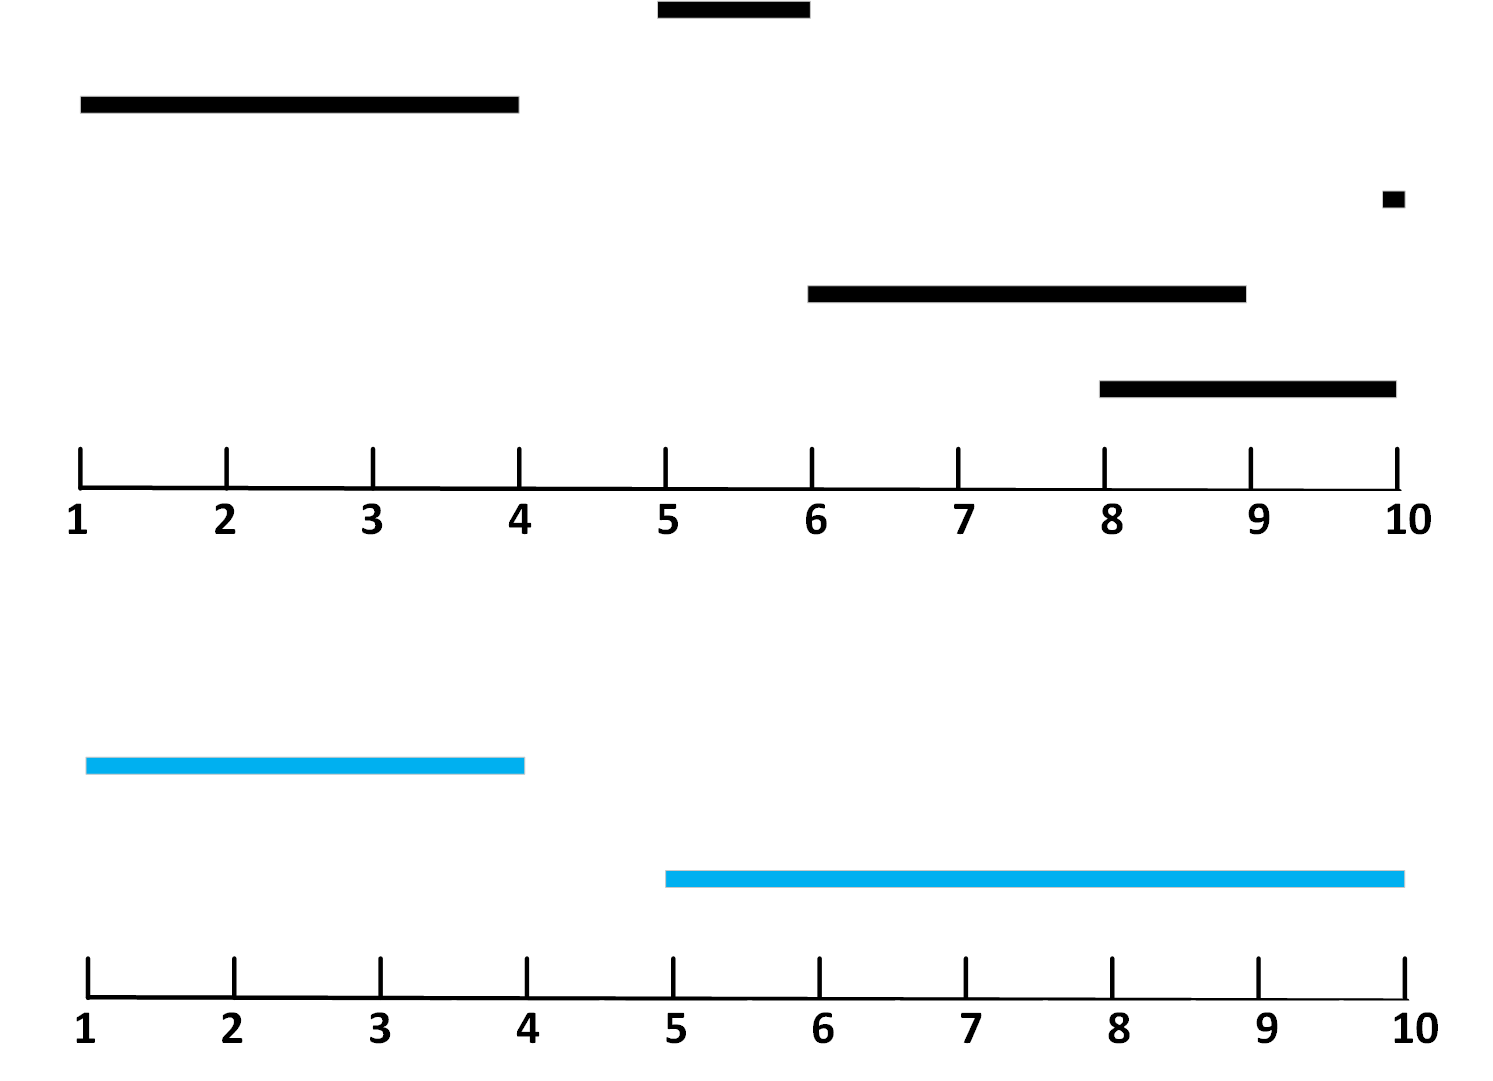
\includegraphics[width=0.9\textwidth]{fig/5-2.png}
    \end{columns}
\end{frame}
\end{document}